% Created 2021-03-31 Wed 11:21
% Intended LaTeX compiler: pdflatex

\documentclass[english]{article}
\usepackage[T1, T2A]{fontenc}
\usepackage[lutf8]{luainputenc}
\usepackage[english, russian]{babel}
\usepackage{minted}
\usepackage{graphicx}
\usepackage{longtable}
\usepackage{hyperref}
\usepackage{xcolor}
\usepackage{natbib}
\usepackage{amssymb}
\usepackage{stmaryrd}
\usepackage{amsmath}
\usepackage{caption}
\usepackage{mathtools}
\usepackage{amsthm}
\usepackage{tikz}
\usepackage{grffile}
\usepackage{extarrows}
\usepackage{wrapfig}
\usepackage{rotating}
\usepackage{placeins}
\usepackage[normalem]{ulem}
\usepackage{amsmath}
\usepackage{textcomp}
\usepackage{capt-of}

\usepackage{geometry}
\geometry{a4paper,left=2.5cm,top=2cm,right=2.5cm,bottom=2cm,marginparsep=7pt, marginparwidth=.6in}
 \usepackage{hyperref}
 \hypersetup{
     colorlinks=true,
     linkcolor=blue,
     filecolor=orange,
     citecolor=black,      
     urlcolor=cyan,
     }

\usetikzlibrary{decorations.markings}
\usetikzlibrary{cd}
\usetikzlibrary{patterns}
\usetikzlibrary{automata, arrows}

\newcommand\addtag{\refstepcounter{equation}\tag{\theequation}}
\newcommand{\eqrefoffset}[1]{\addtocounter{equation}{-#1}(\arabic{equation}\addtocounter{equation}{#1})}


\newcommand{\R}{\mathbb{R}}
\renewcommand{\C}{\mathbb{C}}
\newcommand{\N}{\mathbb{N}}
\newcommand{\rank}{\text{rank}}
\newcommand{\const}{\text{const}}
\newcommand{\grad}{\text{grad}}

\newcommand{\todo}{{\color{red}\fbox{\text{Доделать}}}}
\newcommand{\fixme}{{\color{red}\fbox{\text{Исправить}}}}

\newcounter{propertycnt}
\setcounter{propertycnt}{1}
\newcommand{\beginproperty}{\setcounter{propertycnt}{1}}

\theoremstyle{plain}
\newtheorem{propertyinner}{Свойство}
\newenvironment{property}{
  \renewcommand\thepropertyinner{\arabic{propertycnt}}
  \propertyinner
}{\endpropertyinner\stepcounter{propertycnt}}
\newtheorem{axiom}{Аксиома}
\newtheorem{lemma}{Лемма}
\newtheorem{manuallemmainner}{Лемма}
\newenvironment{manuallemma}[1]{%
  \renewcommand\themanuallemmainner{#1}%
  \manuallemmainner
}{\endmanuallemmainner}

\theoremstyle{remark}
\newtheorem*{remark}{Примечание}
\newtheorem*{solution}{Решение}
\newtheorem{corollary}{Следствие}[theorem]
\newtheorem*{examp}{Пример}
\newtheorem*{observation}{Наблюдение}

\theoremstyle{definition}
\newtheorem{task}{Задача}
\newtheorem{theorem}{Теорема}[section]
\newtheorem*{definition}{Определение}
\newtheorem*{symb}{Обозначение}
\newtheorem{manualtheoreminner}{Теорема}
\newenvironment{manualtheorem}[1]{%
  \renewcommand\themanualtheoreminner{#1}%
  \manualtheoreminner
}{\endmanualtheoreminner}
\captionsetup{justification=centering,margin=2cm}
\newenvironment{colored}[1]{\color{#1}}{}

\tikzset{->-/.style={decoration={
  markings,
  mark=at position .5 with {\arrow{>}}},postaction={decorate}}}
\makeatletter
\newcommand*{\relrelbarsep}{.386ex}
\newcommand*{\relrelbar}{%
  \mathrel{%
    \mathpalette\@relrelbar\relrelbarsep
  }%
}
\newcommand*{\@relrelbar}[2]{%
  \raise#2\hbox to 0pt{$\m@th#1\relbar$\hss}%
  \lower#2\hbox{$\m@th#1\relbar$}%
}
\providecommand*{\rightrightarrowsfill@}{%
  \arrowfill@\relrelbar\relrelbar\rightrightarrows
}
\providecommand*{\leftleftarrowsfill@}{%
  \arrowfill@\leftleftarrows\relrelbar\relrelbar
}
\providecommand*{\xrightrightarrows}[2][]{%
  \ext@arrow 0359\rightrightarrowsfill@{#1}{#2}%
}
\providecommand*{\xleftleftarrows}[2][]{%
  \ext@arrow 3095\leftleftarrowsfill@{#1}{#2}%
}
\makeatother
\author{Ilya Yaroshevskiy}
\date{\today}
\title{Лекция 10}
\hypersetup{
 pdfauthor={Ilya Yaroshevskiy},
 pdftitle={Лекция 10},
 pdfkeywords={},
 pdfsubject={},
 pdfcreator={Emacs 28.0.50 (Org mode 9.4.4)}, 
 pdflang={English}}
\begin{document}

\maketitle
\tableofcontents


\section{Формы хранения матриц}
\label{sec:orgb7858d8}
\begin{definition}
Матрица имеющая достаточное нкбольшое число ненулевых элементов называется \textbf{разреженой}
\end{definition}
\begin{definition}
В ином случае, называется \textbf{плотной}
\end{definition}
Форматы хранения квадратных матриц:
\begin{enumerate}
\item Диагональный
\item Ленточный
\item Профильный
\item Разреженый
\end{enumerate}
Характеристики:
\begin{enumerate}
\item Симметрия матрицы
\item Верхний и нижний треугольники матрицы
\item Ускоренный достпук к строкам матрицы
\end{enumerate}
Будем называть ненулевыми элементами, те которые предполагается хранить в памяти.
\subsection{Диагональный}
\label{sec:org9b928e0}
\begin{center}
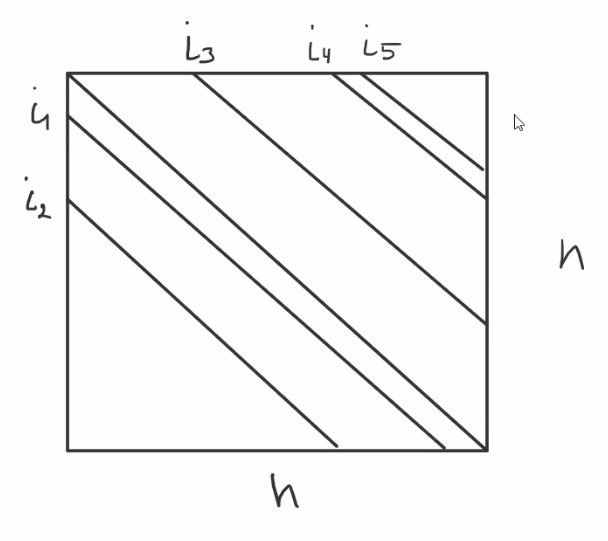
\includegraphics[scale=0.3]{10_1.png}
\end{center}
\begin{itemize}
\item \(n \times n\), где \(n\) --- размерноесть исходной матрицы, \(m\) --- количество ненулевых диагоналей
\end{itemize}
\subsection{Ленточный формат}
\label{sec:orgf688710}
\begin{center}
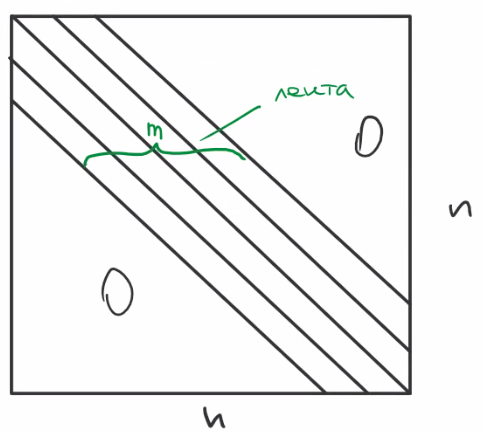
\includegraphics[scale=0.3]{10_2.png}
\end{center}
\(a_{ij} = 0\), если \(|i - j| > k\), \(k\) --- полуширина, \(m = 2k + 1\) --- ширина ленты
\subsection{Профильный формат}
\label{sec:org0124bfe}
\begin{center}
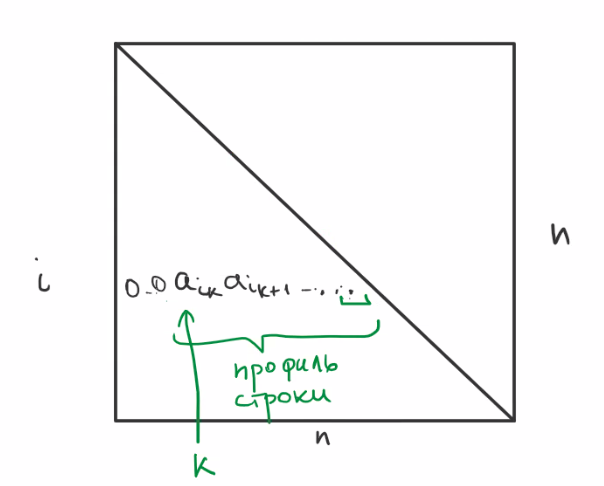
\includegraphics[scale=0.3]{10_3.png}
\end{center}
Обычно хранят несимметричный матрицы. Структуры хранения:
\begin{itemize}
\item Вещественный массив \(di[n]\) --- массив диагональных элементов
\item Вещественные массивы \(al\) --- элементы нижнего треугольника по строками, \(au\) --- эленметы верхнего треугольника по столбцам
\item Целочисленный массив \(ia(k) =\)индекс\color{red}(в нумерации с 1)\color{black}, с которого начинаются элементы \(k\)-ой строки(столбца) в массивах \(al,\ au\). Размерноть равна \(n + 1\), при чем \(ia[n + 1]\) равен индексу первого незанятого элемента в \(al,\ au\), \(a[n + 1] - 1\) --- размерность \(al\) и \(au\).
\end{itemize}
\begin{examp}
\-
\[ \begin{matrix}
a_{11} & & & & & & & & \\
0 & a_{22} & a_{23} & a_{24} & & &  \text{\huge0}& &  \\
0 & a_{32} & a_{33} & 0 & a_{35} & a_{36} & & &  \\
0 & a_{42} & 0 & a_{44} & a_{45} & 0 & a_{47} & &  \\
& & a_{53} & a_{54} & a_{55} & a_{56} & 0 & a_{58} & a_{59} \\
& & a_{63} & 0 & a_{65} & a_{66} & 0 & a_{68} & 0 \\
& & & a_{74} & 0 & 0 & a_{77} & 0 & a_{79} \\
& \text{\huge0}& &  & a_{85} & a_{86} & 0 & a_{88} & 0 \\
& & &  & a_{95} & 0 & a_{97} & 0 & a_{99}
\end{matrix} \]

\[ di = \{a_{11}, a_{22}, a_{33}, a_{44}, a_{55}, a_{66}, a_{77}, a_{88}, a_{99}\} \]
\[ ia = \{1, 1, 1, 2, 4, 6, 9, 12, 15, 19\} \]
\[ al = \{a_{32}, a_{42}, 0, a_{53}, a_{54}, a_{63}, 0, a_{65}, a_{74}, 0, 0, a_{85}, a_{86}, 0, a_{95}, 0, a_{97}, 0\} \]
\[ au = \{a_{23}, a_{24}, 0, a_{35}, a_{45}, a_{36}, 0, a_{56}, a_{47}, 0, 0, a_{58}, a_{68}, 0, a_{59}, 0, a_{79}, 0\} \]
\end{examp}
\end{document}
